\documentclass[12pt]{beamer}
\usetheme{Malmoe}
\usepackage[utf8]{inputenc}
\usepackage[ngerman]{babel}
\usepackage[T1]{fontenc}
\usepackage{amsmath}
\usepackage{amsfonts}
\usepackage{amssymb}
\usepackage{graphicx}
\usepackage{eurosym}
\usepackage{listings}
\usepackage{color}

\author{Philip Caroli}
\title{Arduino für Anfänger}
%\setbeamercovered{transparent} 
%\setbeamertemplate{navigation symbols}{} 
%\logo{} 
%\institute{} 
%\date{} 
%\subject{} 
\begin{document}

\begin{frame}
\titlepage
\end{frame}

\section{Übersicht}
\begin{frame}
\tableofcontents
\end{frame}

\section{Was ist ein Arduino?}

\begin{frame}{Was ist Arduino?}
\begin{itemize}
\item einfach zu bedienende Mikrocontroller-Lernplattform
\item Entwicklungsumgebung mit einheitlichen Befehlen
\begin{itemize}
  \item Unterstützt auch andere Hardware
\end{itemize}
\item 2005 erstes Board entwickelt
\item 2015 Rechtsstreit, neuer Markenname Genuino
\item Unterschiedliche Boards verfügbar
\end{itemize}
\end{frame}

\begin{frame}{Was ist ein Arduino?}
\begin{itemize}
\item Kleine, günstige Platine.
\item Mikrocontroller: Kleiner Rechner.
\item Einfach über USB anzuschließen.
\item Leicht zu programmieren.
\item Reicht für kleine und mittelgroße Projekte
vollkommen aus.
\item Große Community:
\begin{itemize}
  \item Viele Probleme wurden schon gelöst.
  \item Es gibt bewährte Lösungen.
  \item “Arduino-Kompatible” Komponenten.
\end{itemize}
\end{itemize}
\end{frame}

\begin{frame}{Was kann man damit machen?}
\begin{itemize}
\item Mit dem Computer kommunizieren.
\item Leuchtdioden leuchten lassen.
\item Motoren, Lautsprecher u.A. steuern.
\item Temperatur-, Feuchtigkeits-, Lichtsensoren auslesen.
\item Fertige Module benutzen:
\begin{itemize}
  \item Kleine Platine mit modernen Komponenten.
  \item Fertige Beispiele $\rightarrow$ Schnelles Experimentieren.
\end{itemize}
\end{itemize}
\end{frame}

\begin{frame}{Was kann man damit nicht machen?}
\begin{itemize}
\item  Bildbearbeitung und komplexe Programme.
\begin{itemize}
  \item Zu wenig Rechenpower und Speicherplatz
  \item Keine High-Level Komponenten wie USB-Kameras
  \item Besser einen Raspberry verwenden.
\end{itemize}
\item  WLAN- und Bluetoothanwendungen.
\begin{itemize}
  \item Mit Shields möglich, aber teuer.
  \item Besser zB einen ESP8266 verwenden.
\end{itemize}
\end{itemize}
\end{frame}


\section{Elektronik-Grundlagen}

\begin{frame}{Grundlagen}
\begin{itemize}
\item Elektronik-Grundverständnis ist unabdingbar für Arduino-Projekte.
\item Gefahren durch Strom:
\begin{itemize}
  \item Stromschlag: Keine Gefahr bei Niederspannung.
  \item Brandgefahr: Umwahrscheinlich.
  \item Heiße Bauteile: Möglich.
\end{itemize}
\item In diesem Kurs
\begin{itemize}
  \item Nur grobe Einführung in die Materie.
  \item Keine Erklärung der Hintergründe und Funktionsweise.  
\end{itemize}
\end{itemize}
\end{frame}

\begin{frame}{Strom und Spannung}
\begin{itemize}
\item Anschauung zum einfacheren Verständnis:
\begin{itemize}
\item Luftfluß durch ein Rohrsystem.
\item Luftdruck wird durch einen Kompressor in Tank A aufgebaut.
\item Luft entströmt aus Tank A durch ein Rohr in die Umgebung.
\item Je höher der Luftdruck, desto größer der Luftstrom.
\item Wenn keine Druckdifferenz zwischen Tank und Umgebung besteht, strömt keine Luft.
\item Bei doppelter Druckdifferenz ist der Luftstrom doppelt so groß.
\end{itemize}
\end{itemize}
\end{frame}

\begin{frame}{Spannung}
Luftstrom-Äquivalent: Luftdruck
\begin{itemize}
\item Formelzeichen: U, selten V
\item Einheit: Volt [V]
\item Wichtig ist immer die Spannungsdifferenz.
\item Meist wird die Spannungsdifferenz auf die Masse bezogen.
\begin{itemize} %TODO Fix format
  \item 5V bedeutet also, dass die Spannung 5V über der Masse liegt.
  \item Luftstrom-Äquivalent: Umgebungsdruck.
\end{itemize}
\item Auch negative Spannungen (zur Masse) sind möglich.
\item Spannung kann entweder konstant anliegen (Gleichspannung, DC) oder mit einer bestimmten Frequenz (Wechselspannung, AC) ihre Polung wechseln.
\item Hohe Spannungen wie 230 V AC sind lebensgefährlich.
\item Spannungen unter 60V DC gelten als ungefährlich.
\end{itemize}
\end{frame}

\begin{frame}{Strom}
Luftstrom-Äquivalent: Luftstrom
\begin{itemize}
\item Formelzeichen: I
\item Einheit: Ampere [A]
\item Fließt von einer Stelle mit hoher Spannung zu einer mit niedriger Spannung.
\item Benötigt einen elektrischen Leiter zum fließen.
\item Zu hohe Ströme können elektrische Komponenten zerstören.
\item Fließt ein Strom ungehindert von einer Spannugnsquelle zu einer Senke, so spricht man von einem Kurzschluss - Dieser kann die Spannungsquelle beschädigen.
\end{itemize}
\end{frame}

\begin{frame}{Widerstand}
Luftstrom-Äquivalent: Rohr mit Verengung
\begin{itemize}
\item Formelzeichen: R
\item Einheit: Ohm [$\Omega$]
\item Je größer der Widerstand, desto weniger Strom fließt bei einer gegebenen Spannung.
\item Über einem Widerstand fällt bei Durchfluss eine Spannung ab.
\item Wenn ein Widerstand von Strom durchflossen wird, entsteht Wärme.
\end{itemize}
\end{frame}

\begin{frame}{Ohm'sches Gesetz}
Das Ohm’sche Gesetz beschreibt den Zusammenhang zwischen Widerstand, Spannung und Stromstärke:
%TODO Formel einfügen
\begin{itemize}
\item Eselsbrücke zum merken: Rudi $\rightarrow$  R gleich U durch I
\item Andere Formen: $I = U * R$ , $U = R * I$
\item Wichtigste Formel in der Elektrotechnik
\end{itemize}
\end{frame}

\begin{frame}{Kondensator}
Luftstrom-Äquivalent: Gasbehälter mit Membran
\begin{itemize}
\item Formelzeichen: C
\item Einheit: Farad [F]
\item Speichert Energie in einem elektrischen Feld.
\item Je höher die anliegende Spannung, desto mehr Energie wird gespeichert.
\item Werden oft zur Glättung von Spannungen verwendet.
\item Elektrolytkondensatoren (Elkos) haben eine Polarität: Bei negativer Spannung explodieren sie.
\end{itemize}
\end{frame}

\begin{frame}{Induktivität}
Luftstrom-Äquivalent: Turbine mit Schwungrad
\begin{itemize}
\item Formelzeichen: L
\item Einheit: Henry [H]
\item Speichern Energie in einem elektrischen Feld.
\begin{enumerate}
\item Feld wird aufgebaut: Hoher Widerstand.
\item Feld ist aufgebaut: Niedriger Widerstand.
\item Feld wird abgebaut: Spannungsdifferenz wird erzeugt.
\end{enumerate}
\item Werden in Elektromotoren verwendet.
\end{itemize}
\end{frame}

\begin{frame}{Dioden}
Luftstrom-Äquivalent: Rückschlagventil
\begin{itemize}
\item Leiten Strom nur in einer Richtung.
\item Haben eine Durchlassspannung, unter der sie (fast) nicht leiten.
\item Über ihnen fällt eine Bauartbedingte Spannung ab: Bei Siliziumdioden zB 0,7V.
\item Bei kleinem Spannugnsanstieg vergrößert sich der Durchflussstrom sprunghaft.
\item Bei Durchfluss entsteht Wärme, ähnlich wie bei Widerständen.
\item Werden bei höherer Temperatur leitfähiger $\rightarrow$ Teufelskreis
\item Bei zu viel Wärme werden Dioden zerstört.
\end{itemize}
\end{frame}

\begin{frame}{Leuchtdiode}
\begin{itemize}
\item Sind Dioden, die außer Wärme auch Licht ausstrahlen.
\item Typischer Wirkungsgrad: 20’% $\rightarrow$ 80% der Leistung ist Wärme.
\item “Typische” LEDs sind für einen Stromfluss von 20mA spezifiziert.
\item Haben eine Sperrspannung von 5V.
\item Werden mit einem Vorwiderstand geschützt:
\end{itemize}
\begin{tabular}{|l|l|l|}
Farbe     & Spannung & Vorwiderstand bei 5V \\
\hline
Infrarot  & 1,5V     & 390$\Omega$ \\
Rot       & 1,6V     & 390$\Omega$ \\
Orange    & 2,0V     & 330$\Omega$ \\
Gelb      & 2,2V     & 330$\Omega$ \\
Grün      & 2,1V     & 330$\Omega$ \\
Blau      & 2,9V     & 220$\Omega$ \\
Weiß + UV & 4,0V     & 100$\Omega$ \\
\end{tabular}
\end{frame}

\begin{frame}{(Feldeffekt)Transistor}
Luftfluß-Äquivalent: Druckgesteuertes Ventil
\begin{itemize}
\item Haben 3 Anschlüsse: Gate, Source, Drain.
\item Werden als Schalter verwendet.
\item Schalten durch, sobald an Gate eine Spannung anliegt.
\item Können benutzt werden, um hohe Spannungen und starke Strom zu schalten.
\end{itemize}
\end{frame}

\begin{frame}{Der Arduino als elektrisches Bauteil}
\begin{itemize}
\item Stromversorgung über USB-Kabel: 5V, maximal 500mA.
\item Stromversorgung über VIn-Pin: 6 bis 20V.
\item Stromversorgung über 5V-Netzteil: maximal 1A.
\item Erzeugt eine 3,3V-Spannung, Belastbarkeit 50mA.
\item Besitzt 22 digitale Eingabe/Ausgabe-Pins:
\begin{itemize}
\item Eingabe: Können messen, ob eher Masse oder 5V anliegt.
\item Haben einen einschaltbaren hochohmigen Widerstand nach 5V
\item Ausgabe: Können Masse oder 5V oder nichts ausgeben.
\item Vertragen jeweils maximal 40mA, alle zusammen nicht mehr als 200mA.
\end{itemize}
\end{itemize}
\end{frame}

\begin{frame}{Die Anschlüsse des Arduino Nano}
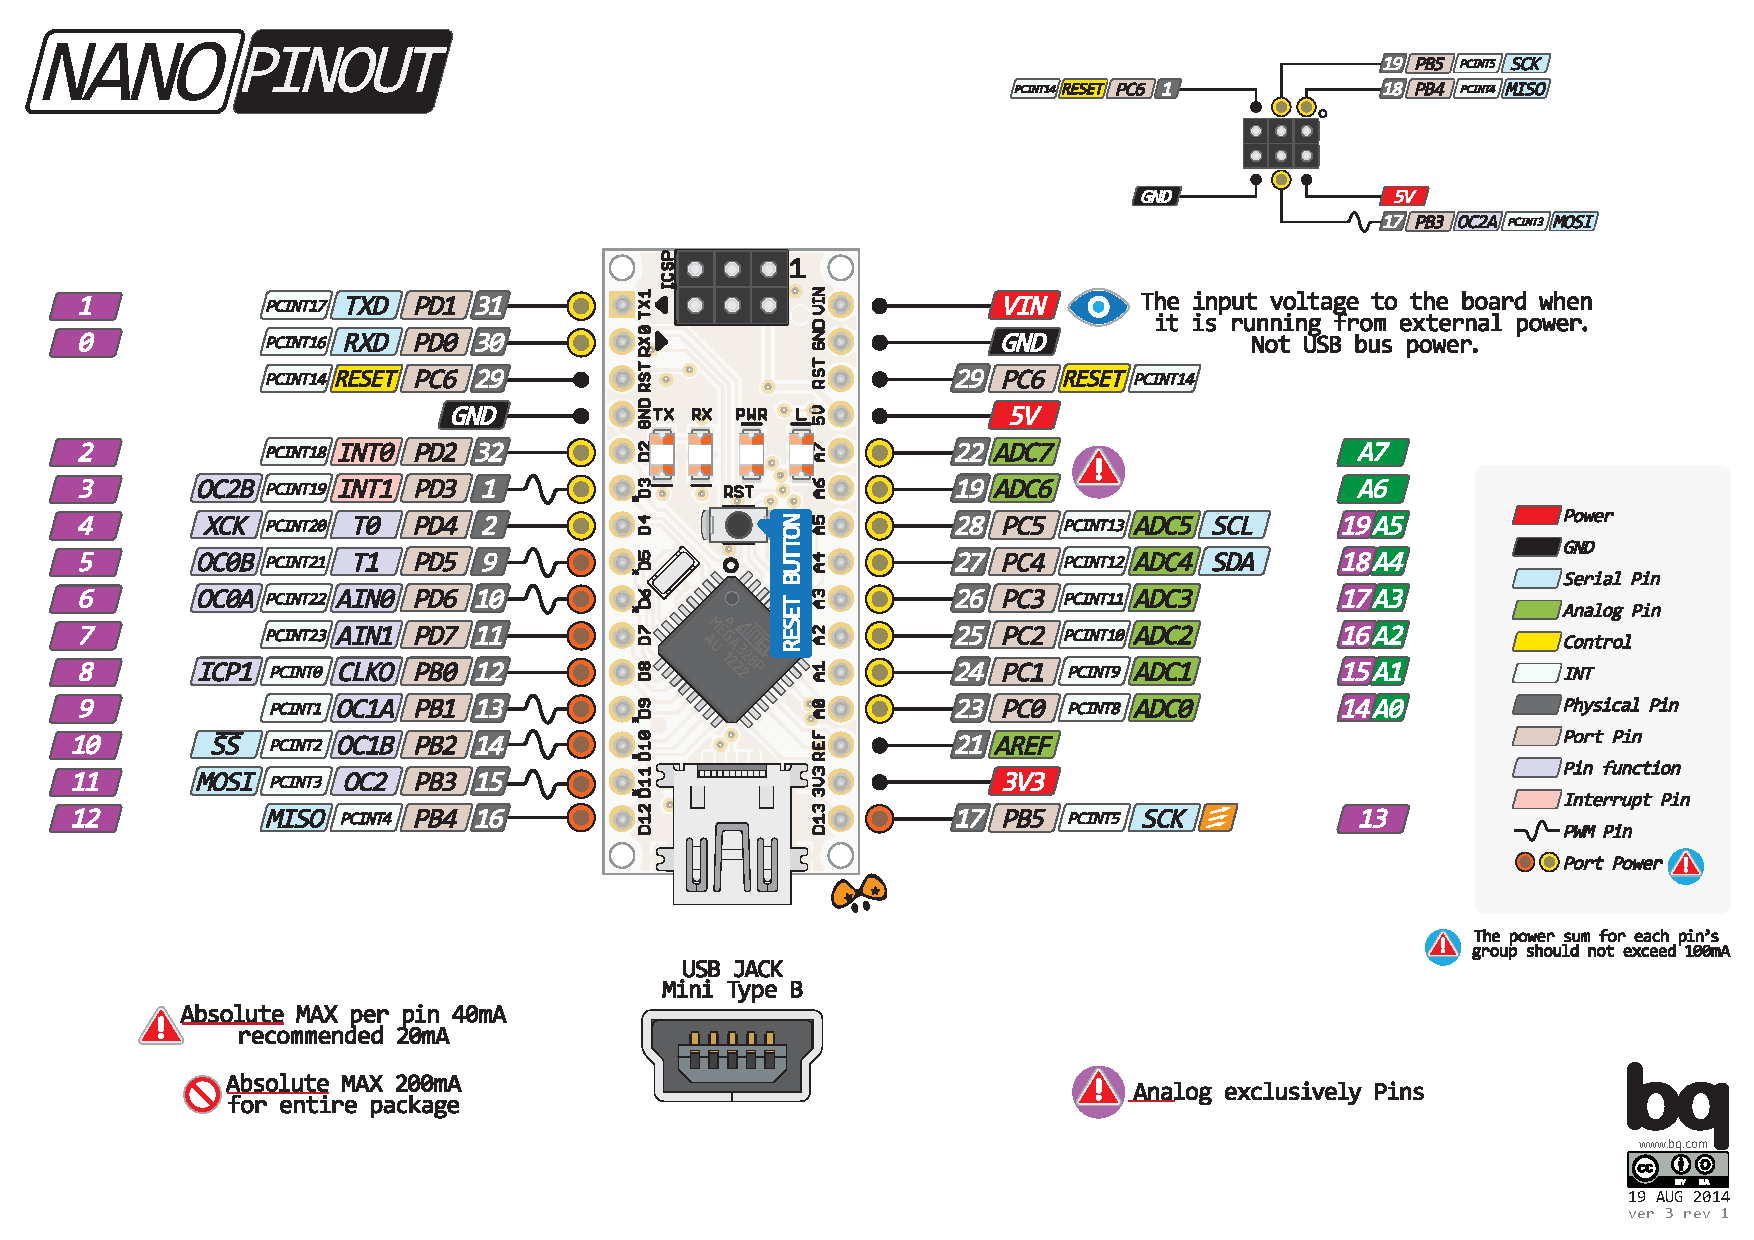
\includegraphics[scale=0.3]{Bilder/nano_pinout.pdf}
\end{frame}

%\begin{frame}{Löten}
\begin{itemize}
\item Der Arduino Nano muss noch zusammengelötet werden.
\item Dafür die Lötstation auf 300 C einstellen und eine Minute warten.
\item Die langen Stiftleisten von unten einstecken, sodass der USB-Anschluss oben liegt.
\item Mit dem Lötkolben eine Lötstelle 2-3 Sekunden erwärmen.
\item Lötzinn hinzufügen, 2-3 Sekunden warten.
\item Lötkolben wegnehmen, Lötstelle begutachten.
\item Die Lötstelle muss glänzen und den Pin mit der Platine verbinden.
\end{itemize}
%\end{frame}

\section{Programmiergrundlagen}

\begin{frame}{Microcontroller-Programmierung}
\begin{itemize}
\item Einsatz von Cross-Compilern.
\item Wird von der Arduino IDE automatisch geregelt:
\begin{enumerate}
  \item Code wird auf Korrektheit geprüft.
  \item Einzelne Dateien werden kompiliert.
  \item Dateien und Bibliotheken werden zu einem "Hex-File" verlinkt.
  \item Der Mikrocontroller wird in den Programmiermodus versetzt.
  \item Das Hex-File wird hochgeladen und überprüft.
  \item Der Mikrocontroller wird neugestartet.
\end{enumerate}
\end{itemize}
\end{frame}


\begin{frame}{Die Entwicklungsumgebung}
\begin{itemize}
\item Kann unter https://www.arduino.cc/en/Main/Software heruntergeladen werden.
\item ist für Windows, Linux und MocOS verfügbar.
\item Ubuntu-Packetverwaltung beinhaltet nur alte Version - bei Problemen trotzdem \texttt{sudo apt-get install arduino-core} ausführen.
\item Windows: Unbedingt auch die USB-Treiber installieren lassen.
\item Beinhaltet viele nützliche Beispiele.
\item Programme werden meist “Sketch” (Skizze) genannt.
\item USB-Treiber für Arduinos werden auch mitinstalliert
\end{itemize}
\end{frame}

\begin{frame}{Test der Installation}
\begin{enumerate}
\item Arduino IDE starten.
\item Datei $\rightarrow$ Beispiele $\rightarrow$ 01.Basics $\rightarrow$ Blink auswählen.
\item Beide delay(1000); in delay(250); ändern.
\item Tools $\rightarrow$ Boards $\rightarrow$ Arduino Nano auswählen.
\item Unter Tools $\rightarrow$ Port den richtigen / einzigen Port wählen.
\item Mit Sketch $\rightarrow$ Upload oder [Strg]+[U] den Sketch auf den Arduino laden.
\item Der Sketch muss nicht gespeichert werden.
\item Die LED auf dem Arduino blinkt jetzt schneller
\end{enumerate}
\end{frame}

\begin{frame}{Prgrammaufbau}
\begin{itemize}
\item Ein Programm ist eine Liste von Befehlen.
\item Jeder Befehl muss korrekt geschrieben sein.
\item Jeder vollständige Befehl wird mit einem Semikolon beendet.
\item Grundrechenarten können direkt benutzt werden.
\item Befehle sind meist Zuweisungen, zB A = A + B;
\item Befehle, die andere Teilprogramme aufrufen, bestehen aus einem Text und einem Klammernpaar.
\item In den Klammern werden die Parameter des Befehls angegeben.
\item Der Befehl gibt einen oder keinen Wert zurück.
\end{itemize}
\end{frame}

\begin{frame}{Syntax}
%TODO 
\end{frame}

\begin{frame}{Variablen}
\begin{itemize}
\item Eine Variable muss vor der Verwendung deklariert werden:
TYP NAME;
\item Danach wird sie initialisiert: NAME = WERT;
\item Beides kann kombiniert werden: TYP NAME = WERT;
\item Basis-Typen:
\end{itemize}
\begin{tabular}{|l|l|l|l|}
Type   & Beschreibung    & Wertebereich   & Beispiel \\
\hline
int    & ganze Zahl      & -32768 - 32767 & 24000    \\
float  & Fließkommazahl  & $\pm$ 3.4028235E38  & 3.14     \\
char   & ganze Zahl      & -128 - 127     & -12      \\
byte   & ganze Zahl      & 0 - 255        & 128      \\
string & Zeichenkette    &                & “Hallo”  \\
bool   & true oder false & true, false    & false    \\
\end{tabular}
\end{frame}

\begin{frame}{Bedingungen}
Klassische “Wenn, dann”-Abfragen.

\end{frame}

\begin{frame}{Arduino-Pins ansteuern}
\begin{itemize}
\item \texttt{pinMode(1, INPUT);} Der Pin gibt keine Ausgangsspannung aus.
\item \texttt{pinMode(1, OUTPUT);} Der Pin gibt eine Ausgangsspannung aus.
\item \texttt{digitalWrite(1, LOW);} Die Ausgangsspannung ist Masse (0V).
\item \texttt{digitalWrite(1, HIGH);} Die Ausgangsspannung ist 5V.
\item \texttt{variable = digitalRead(1);} Die Variable ist true, wenn 5V am
Pin anliegt, und false wenn Masse anliegt.
\end{itemize}
\end{frame}

\begin{frame}{Bibliotheken}
\begin{itemize}
\item Bibliotheken beinhalten fertige Softwarebausteine und Beispiele, wie sie verwendet werden können.
\item Sie können unter Sketch $\rightarrow$ Bibliothek hinzufügen $\rightarrow$ Bibliothek verwalten installiert werden.
\end{itemize}
\end{frame}

\begin{frame}{Beispiel: Reaktionszeit-Tester}
\begin{itemize}
\item Kleines alternatives Beispielprogramm.
\item Eine LED geht in einer zufälligen Zeit an.
\item Der Benutzer drückt als Reaktion auf eine Taste.
\item Wenn er schnell genug ist, leuchtet die LED 2s schnell blinkend.
\item Wenn nicht, passiert nichts.
\end{itemize}
\end{frame}


\end{document}
